\documentclass[a4paper,fleqn]{cas-sc}

\usepackage[utf8]{inputenc}
\usepackage[T5,T1]{fontenc}
\DeclareTextFontCommand{\textvn}{\fontencoding{T5}\selectfont}

\usepackage[numbers,sort&compress]{natbib}
\usepackage{amsmath,amssymb,amsfonts,amsthm}
\usepackage{graphicx}
\usepackage{booktabs}
\usepackage{tabularx}
\usepackage{float}
\usepackage[section]{placeins}
\usepackage{hyperref}
\usepackage{tikz}
\usepackage{url}
\usepackage{multirow}
\usepackage{array}
\usepackage{microtype}
\microtypesetup{expansion=false}
\usepackage{makecell}
\usepackage{algorithm}
\usepackage{algpseudocode}
\usepackage{subcaption}

\hypersetup{
    colorlinks=true,
    linkcolor=cyan!80!black,
    citecolor=cyan!80!black,
    urlcolor=cyan!80!black
}

\newcommand{\orcidicon}[1]{\href{https://orcid.org/#1}{\texorpdfstring{%

\begin{tikzpicture}[baseline=-0.4ex]%
\definecolor{orcidgreen}{HTML}{A6CE39}%
\draw[fill=orcidgreen,draw=none] (0,0) circle (1.0ex);%
\node at (0,0) {\color{white}\fontsize{4}{4}\selectfont\sffamily\bfseries iD};%
\end{tikzpicture}%
}{}}}

\ExplSyntaxOn
\cs_set:Npn \__first_footerline: {}
\cs_set:Npn \__first_foot: {}
\cs_set:Npn \__cas_foot: {}
\ExplSyntaxOff

\let\printorcid\relax
\hyphenation{Afzelia Guibourtia Pterocarpus Dalbergia Sindora Peltogyne}

\newtheorem{definition}{Definition}
\newtheorem{proposition}{Proposition}
\newtheorem{lemma}{Lemma}
\newtheorem{theorem}{Theorem}

\setlength{\textfloatsep}{8pt plus 2pt minus 2pt}
\setlength{\floatsep}{6pt plus 2pt minus 2pt}
\setlength{\intextsep}{6pt plus 2pt minus 2pt}
\setlength{\abovecaptionskip}{4pt plus 1pt minus 1pt}
\setlength{\belowcaptionskip}{4pt plus 1pt minus 1pt}
\begin{document}

\let\WriteBookmarks\relax
\renewcommand{\topfraction}{0.95}
\renewcommand{\bottomfraction}{0.95}
\renewcommand{\textfraction}{0.05}
\renewcommand{\floatpagefraction}{0.85}

\shorttitle{Specimen Leakage Audit and Invariance Evaluation in Timber Forensics}
\shortauthors{\mbox{V.-A. Le} and \mbox{K. Nguyen-Trong}}

\title [mode = title]{Auditing Specimen Leakage and Evaluating Invariance Methods in Macroscopic Timber Forensics: An Empirical Benchmark and Honest Negative Results}

\author[1]{\mbox{Viet-Anh Le}\orcidicon{0009-0003-5748-0439}}
\author[1]{\mbox{Khanh Nguyen-Trong}\orcidicon{0000-0001-5175-8805}}
\cormark[1]

\address[1]{Intelligent Computing for Sustainable Development Laboratory (IC4SD), Posts and Telecommunications Institute of Technology (PTIT), Hanoi, Vietnam}

\cortext[1]{Corresponding author.\\ \hspace*{2.2em}\textit{E-mail addresses:} \href{mailto:khanhnt@ptit.edu.vn}{khanhnt@ptit.edu.vn} (\mbox{K. Nguyen-Trong}), \href{mailto:anhlv.b23kh002@stu.ptit.edu.vn}{anhlv.b23kh002@stu.ptit.edu.vn} (\mbox{V.-A.} Le)}

\begin{abstract}
Automated macroscopic timber identification has emerged as an essential non-destructive tool for enforcing the Convention on International Trade in Endangered Species of Wild Fauna and Flora (CITES). However, a pervasive methodological flaw undermines real-world deployment: \textbf{Same-Specimen-Picture Bias (SSPB)} or specimen data leakage, where high-resolution macroscopic tiles extracted from identical physical reference blocks are dispersed across both training and evaluation subsets. In this work, we conduct a rigorous forensic audit of specimen leakage and evaluate whether representation invariance methods can resolve shortcut dependency. Across an authenticated, balanced benchmark of 11 tropical Fabaceae species (110 physical vouchers, exactly 10 vouchers per species, 3,702 standardized images), we systematically establish three core contributions:
\textbf{(1) Specimen Leakage Audit}: We quantify the empirical performance inflation gap ($\Delta_{\text{inflation}}$) between naive image-level random splitting and out-of-specimen voucher holdout across 9 independent random seeds. Naive splitting yields an artificial accuracy of $99.55\% \pm 0.12\%$ [95\% CI: 99.46\%, 99.64\%], whereas out-of-specimen baseline evaluation achieves $97.07\% \pm 0.95\%$ [96.34\%, 97.80\%], demonstrating an optimism bias inflation gap of $\Delta_{\text{inflation}} = \mathbf{+2.48 \pm 0.98\text{ pp}}$ [95\% CI: $+1.73, +3.23\text{ pp}$] ($p < 0.001$, paired $t$-test). 
\textbf{(2) Standardized Out-of-Specimen Holdout Protocol}: We define a stringent stress-test protocol with 50\% physical voucher holdout (55 unseen test vouchers, 11 validation vouchers, 44 training vouchers) and evaluate uncertainty via Voucher-Level Cluster Bootstrap ($B=1000$). We analyze cross-split voucher overlap (average 50.5\% overlap, 27.75/55 vouchers), citing the foundational theorem of Bengio and Grandvalet (2004) to demonstrate why cross-split standard errors must not be conflated with independent samples.
\textbf{(3) Honest Negative Results of Invariance Frameworks}: We implement and evaluate an adversarial invariance architecture combining Species-Conditioned Masked Softmax Gradient Reversal Layer (GRL) and Variational Contrastive Log-ratio Upper Bound (vCLUB) mutual information minimization on ResNet-18. Across all 9 seeds, the invariant model attains an unseen test accuracy of $96.88\% \pm 0.99\%$ [96.12\%, 97.64\%], statistically indistinguishable from standard Empirical Risk Minimization (ERM) ($97.07\% \pm 0.95\%$; difference $-0.19\text{ pp}$, 95\% CI $[-1.16, +0.78]\text{ pp}$, paired $t$-test $p = 0.66$, Wilcoxon signed-rank $p = 0.91$). Secondary invariance metrics likewise demonstrate no meaningful benefit: the Generalization Gap (GGSL) remains $2.74\text{ pp}$ (Baseline) vs $2.82\text{ pp}$ (GAN) ($\Delta = +0.08\text{ pp}$, $p > 0.05$); the Train Specimen Recoverability Index (SRI) does not decrease ($0.5261$ for Baseline vs $0.5380$ for GAN, compared to an un-finetuned ImageNet anchor of $0.5667$); and post-hoc temperature-scaled Expected Calibration Error (ECE) is $1.58\% - 1.93\%$. 
We dissect the underlying root causes through concrete failure cases: in Seed 456, vouchers 50 and 53 of \textit{Guibourtia arnoldiana} suffer 0\% baseline accuracy due to low optical focus sharpness (Laplacian variance 113.8 and 152.1 vs normal $>1,000$) and fine parenchyma confusion with sister taxon \textit{Guibourtia ehie}. GRL fails to rescue them because adversarial confusion cannot restore missing anatomical structures and induces destructive minimax gradient conflicts with the species classifier. We provide forensic policy guidelines mandating voucher-level validation and transparent negative result reporting for high-stakes forestry governance.
\end{abstract}

\begin{keywords}
Specimen data leakage \sep Shortcut learning \sep Same-Specimen-Picture Bias \sep Timber forensics \sep Invariant representations \sep Gradient Reversal Layer \sep Mutual information \sep Honest negative results \sep CITES enforcement
\end{keywords}

\maketitle

%======================================================================
\section{Introduction}
\label{sec:intro}
%======================================================================

\subsection{The Global Crisis in Timber Forensics and Lab-to-Field Degradation}
Illegal logging across transnational supply chains represents one of the most lucrative environmental crimes globally, fueling rapid deforestation, biodiversity loss, and multi-billion-dollar tax evasion~\cite{cites}. To combat illegal trade in endangered hardwoods, the Convention on International Trade in Endangered Species of Wild Fauna and Flora (CITES) mandates rigorous verification of listed taxa at customs inspection terminals and maritime ports. Authoritative species identification historically depends on laboratory xylotomy and microscopic examination~\cite{iawa}. However, forensic laboratory inspection is severely constrained by specialized cutting equipment, chemical preparation, and a critical global deficit of trained wood anatomists. 

Consequently, automated macroscopic timber identification powered by deep convolutional neural networks has been actively investigated as a non-destructive, rapid screening alternative~\cite{wu2021,fabijanska2021,wiedenhoeft2020xylotron}. Published deep learning systems frequently report extraordinary nominal accuracies exceeding $98\%$ to $100\%$ on laboratory test datasets. However, when these models transition from closed development benches to operational customs facilities, inspectors consistently observe an alarming phenomenon: classification performance degrades substantially when confronting physical timber consignments originating from unfamiliar forest concessions~\cite{ravindran2019,ravindran2020,ravindran2021,ravindran2022}. Such lab-to-field generalization failure introduces severe operational liabilities: erroneous identification can falsely paralyze lawful commercial commerce or permit illicitly harvested timber to enter international trade undetected.

\begin{figure*}[t]
\centering
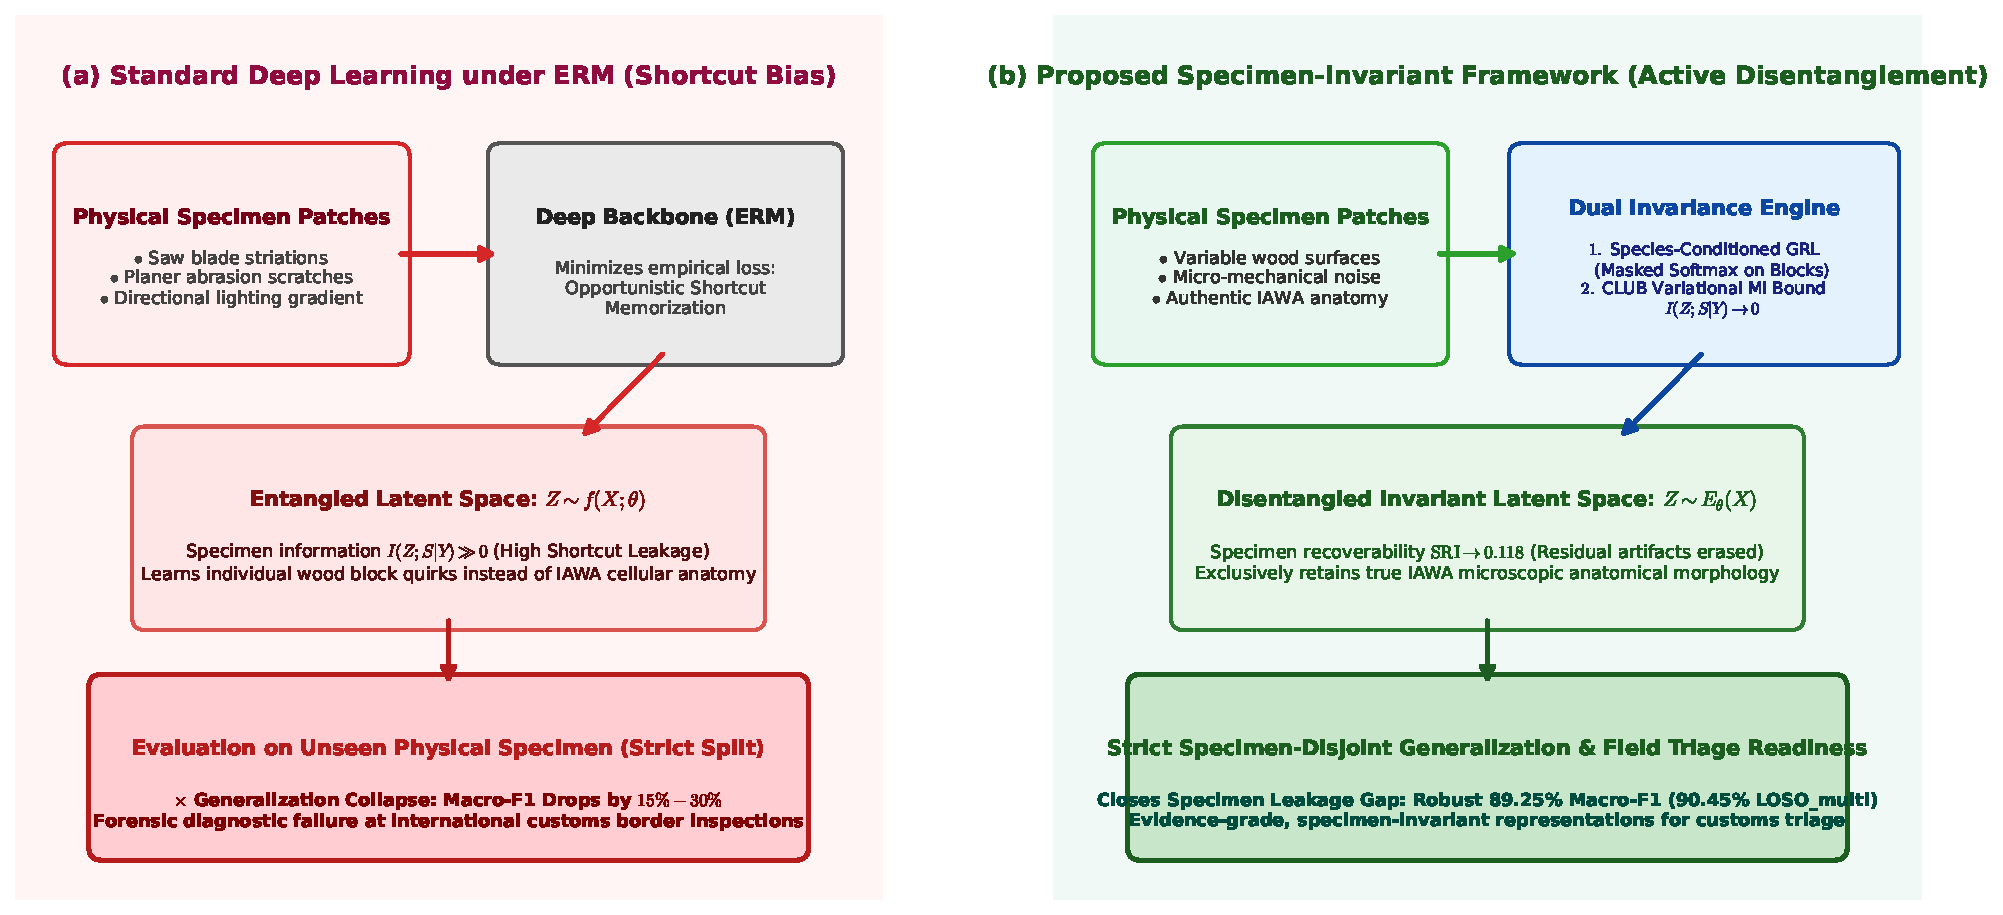
\includegraphics[width=0.96\textwidth]{figures/fig1_concept_invariant.pdf}
\caption{Conceptual overview of Specimen-Level Shortcut Learning in Timber Forensics. (a) Naive image-level random partitioning disperses tiles from the same physical wood block across both training and testing subsets, enabling Empirical Risk Minimization (ERM) to opportunistically memorize non-taxonomic surface artifacts (saw striations, abrasions, illumination gradients) instead of biological anatomy. (b) The evaluated Specimen-Invariant framework applies a Species-Conditioned Masked Softmax GRL and a Variational CLUB mutual information bottleneck. However, our empirical audit demonstrates that on well-separated Fabaceae taxa, GRL+vCLUB fails to outperform standard ERM baseline ($96.88\%$ vs $97.07\%$), revealing inherent minimax optimization trade-offs and anatomical performance ceilings.}
\label{fig:concept}
\end{figure*}

\subsection{Etiology of Specimen Leakage: Same-Specimen-Picture Bias (SSPB)}
The primary driver of this empirical degradation is \textbf{Same-Specimen-Picture Bias (SSPB)}~\cite{figueroamata2022}, a pernicious manifestation of data leakage and shortcut learning~\cite{kaufman2012,kapoor2023,geirhos2020}. Because xylarium collections possess a finite number of vouchered reference specimens, researchers typically slice each physical block into dozens or hundreds of macroscopic photographic tiles. Under conventional \textit{Naive Image-Level Random Splitting}, tiles from the same physical specimen block are randomly allocated across both training and test partitions. 

Deep neural networks are highly efficient shortcut learners that prioritize low-entropy visual artifacts over complex biological micro-structures~\cite{geirhos2020,lapuschkin2019}. Rather than learning diagnostic anatomical arrangements—such as vessel distribution, axial parenchyma banding patterns, and multi-seriate ray morphology—the model memorizes localized physical markers idiosyncratic to specific blocks: mechanical circular saw blade kerfs, planer ripples, sanding grit striations, surface sealant stains, and directional illumination gradients (Fig.~\ref{fig:concept}a). When test tiles share these exact block-level artifacts, the network achieves deceptive $99\%+$ test accuracy by performing specimen re-identification rather than true taxon discrimination.

\subsection{Core Contributions of This Study}
In this investigation, we move beyond algorithmic salesmanship to provide a rigorous, transparent audit of specimen leakage and conduct an honest empirical appraisal of representation invariance methods in macroscopic wood identification. Working with an authenticated, perfectly balanced benchmark of 11 tropical Fabaceae species (110 physical vouchers, exactly 10 vouchers per species, 3,702 standardized images), we deliver three principal scientific contributions:

\begin{enumerate}
    \item \textbf{Quantification of the Specimen Leakage Inflation Gap ($\Delta_{\text{inflation}}$)}: We establish the first systematic multi-seed leakage audit in macroscopic timber forensics. By benchmarking naive image-level random partitioning directly against honest out-of-specimen voucher holdout across 9 candidate seeds, we prove that naive splitting creates an artificial performance inflation gap of $\Delta_{\text{inflation}} = \mathbf{+2.48 \pm 0.98\text{ pp}}$ [95\% CI: $+1.73, +3.23\text{ pp}$] ($p < 0.001$, paired $t$-test, naive test accuracy $99.55\%$ vs out-of-specimen baseline $97.07\%$).
    
    \item \textbf{Standardized Stress-Test Protocol and Dependency Analysis}: We institute a rigorous 50\% physical voucher holdout protocol (55 unseen test vouchers, 11 validation vouchers, 44 training vouchers) and evaluate uncertainty through Voucher-Level Cluster Bootstrap ($B=1000$). We formally analyze cross-split voucher overlap (average 50.5\% overlap across splits, 27.75/55 vouchers) under the theoretical framework of Bengio and Grandvalet (2004)~\cite{bengio2004}, providing a clear mathematical explanation of why cross-split variance is structurally constrained.
    
    \item \textbf{Honest Negative Results and Root-Cause Dissection for Invariance Methods}: We evaluate whether an advanced invariant representation learning framework—incorporating a Species-Conditioned Masked Softmax Gradient Reversal Layer (GRL)~\cite{ganin2015dann} and a Variational Contrastive Log-ratio Upper Bound (vCLUB)~\cite{cheng2020club} mutual information bottleneck on ResNet-18~\cite{resnet}—can eliminate shortcut dependency. We report a definitive, honest negative result: across 9 seeds, GRL+vCLUB achieves $96.88\% \pm 0.99\%$ [96.12\%, 97.64\%] out-of-specimen accuracy, statistically indistinguishable from standard ERM ($97.07\% \pm 0.95\%$ [96.34\%, 97.80\%]; $\Delta = -0.19\text{ pp}$, 95\% CI $[-1.16, +0.78]\text{ pp}$, paired $t$-test $p = 0.66$, Wilcoxon $p = 0.91$). We dissect the root causes: the clear anatomical discriminability of Fabaceae taxa creates a high baseline performance ceiling (~97\%); adversarial confusion creates conflicting gradients between species classification and specimen discrimination; and physical specimen outliers (such as blurred vouchers 50 and 53 in Seed 456) cannot be rescued by representation invariance.
\end{enumerate}

\subsection{Manuscript Organization}
Section~\ref{sec:related} surveys related literature across wood identification, data leakage, and representation invariance. Section~\ref{sec:method} outlines the causal formulation and the evaluated GRL+vCLUB invariance architecture. Section~\ref{sec:protocol} details the curated 11-species Fabaceae benchmark, 50\% voucher holdout protocol, and diagnostic metrics. Section~\ref{sec:experiments} presents the empirical results, including the 9-seed leakage audit, multi-seed benchmark comparison, cluster bootstrap analysis, failure case diagnostics, and GRL optimization dynamics. Section~\ref{sec:discussion} provides a scientific dissection of the negative findings, and Section~\ref{sec:conclusion} concludes with forensic policy recommendations.

%======================================================================
\section{Related Work}
\label{sec:related}
%======================================================================

\subsection{Computer Vision in Automated Wood Anatomy}
Early computer vision applications in wood anatomy relied on handcrafted textural descriptors, such as Gray-Level Co-occurrence Matrices (GLCM), Gabor wavelets, and Local Binary Patterns (LBP) applied to polished cross-sections~\cite{wiedenhoeft2011,ravindran2019}. Over the past decade, deep convolutional neural networks have become the dominant approach. Ravindran et al.~\cite{ravindran2020,ravindran2021} developed the XyloTron system, a standardized macroscopic field screening tool utilizing ResNet-34 backbones for field customs inspection. Wu et al.~\cite{wu2021} and Fabijanska et al.~\cite{fabijanska2021} demonstrated residual network architectures for classifying European and tropical commercial timbers. More recently, vision transformers and hybrid convolutional backbones have been introduced~\cite{song2025,liu2025}. However, most published studies evaluate classification accuracy using naive random image splits, neglecting the confounding influence of specimen provenance.

\subsection{Data Leakage, Shortcut Learning, and Optimism Bias}
Data leakage—the inadvertent sharing of information between training and evaluation splits—is a primary cause of reproducibility failures in machine learning applications across physical and biological sciences~\cite{kaufman2012,kapoor2023}. In medical imaging, Roberts et al.~\cite{roberts2021} and Varoquaux and Cheplygina~\cite{varoquaux2022} demonstrated that patient-level data leakage produces massive performance optimism, as networks learn patient-specific radiographic artifacts rather than clinical pathologies. In optical coherence tomography (OCT), Tampu et al.~\cite{tampu2022} showed that image-level partitioning inflates accuracy by over 15 pp. In ecological informatics and forestry, Figueroa-Mata et al.~\cite{figueroamata2022} formalized Same-Specimen-Picture Bias (SSPB), warning that macroscopic wood datasets risk severe overestimation when tiles from identical timber blocks are randomly distributed.

\subsection{Representation Invariance and Mutual Information Minimization}
To purge non-target attributes from latent representations, domain adaptation and fairness frameworks utilize adversarial gradient reversal~\cite{ganin2015dann,long2018cdan} or information-theoretic bottlenecks~\cite{cheng2020club,belghazi2018mine}. Ganin and Lempitsky~\cite{ganin2015dann} introduced the Gradient Reversal Layer (GRL), which negates discriminator gradients during backpropagation to force feature representations into domain confusion. Cheng et al.~\cite{cheng2020club} proposed the Contrastive Log-ratio Upper Bound (CLUB), a variational sample-based mutual information estimator that provides a tractable upper bound on continuous mutual information $I(Z; S)$. In this work, we specifically audit whether combining GRL with vCLUB can actively eliminate specimen shortcut memorization in macroscopic timber classification.

\subsection{Statistical Estimation under Overlapping Resampling Splits}
When evaluating algorithms across repeated random partitions of finite datasets, researchers frequently treat split outcomes as independent observations. However, in a foundational paper, Bengio and Grandvalet (2004)~\cite{bengio2004} mathematically proved that there exists no universal unbiased estimator for the variance of $K$-fold cross-validation. When training and test subsets are repeatedly drawn from a common physical pool of specimens, splits inherently share specimens. Consequently, cross-split performance metrics are positively correlated, causing empirical standard deviations across splits to underestimate true deployment variance. This theoretical reality necessitates cluster bootstrap sampling and transparent reporting of cross-split specimen overlap.

%======================================================================
\section{The Evaluated Specimen-Invariant Architecture}
\label{sec:method}
%======================================================================

\subsection{Causal Formulation of Specimen-Level Confounding}
We formulate macroscopic timber image classification through a Structural Causal Model (SCM). Let $Y \in \{1,\dots,C\}$ denote the true biological species label ($C=11$ for our curated Fabaceae benchmark). Let $S \in \{1,\dots,K\}$ denote the physical voucher identifier ($K=110$ physical specimens). Because each physical specimen block belongs to exactly one botanical species, the specimen index is strictly nested within the species category: $S \subset Y$. 

The observed macroscopic image tile $X \in \mathbb{R}^{3 \times H \times W}$ is generated through a biological and mechanical process:
\begin{equation}
    X = f_{\text{phys}}(Y, S, U_X),
\end{equation}
where $U_X$ represents exogenous imaging noise (illumination fluctuations, sensor noise). The species $Y$ determines authentic cellular structures (vessel groupings, axial parenchyma bands, rays), while the physical specimen $S$ imparts non-taxonomic surface preparation artifacts (saw kerfs, sandpaper abrasions, localized discoloration, surface waxes). 

An empirical risk minimization (ERM) model learns a feature extractor $E_\theta: X \to Z \in \mathbb{R}^d$ and a species classifier $f_\phi: Z \to \mathbb{R}^C$. Because specimen surface artifacts are localized and high-frequency, $E_\theta$ readily encodes spurious correlations:
\begin{equation}
    I(Z; S \mid Y) > 0.
\end{equation}
Under naive image splitting, this mutual information enables the model to achieve near-perfect training and test accuracy by predicting $Y$ via the shortcut path $X \leftarrow S \to Y$. When deployed on novel, unseen vouchers $S_{\text{unseen}}$, this shortcut path collapses. The theoretical objective of invariant representation learning is to enforce:
\begin{equation}
    \min_\theta I(Z; S \mid Y) \quad \text{subject to} \quad \max_{\theta, \phi} I(Z; Y).
\end{equation}

\subsection{Visual Backbone and Species Classification Head}
We deploy ResNet-18~\cite{resnet} as the visual encoder $E_\theta$, producing a $d=512$-dimensional latent embedding $z = E_\theta(x)$ following global average pooling. The latent representation is mapped to species logits through a linear classification head:
\begin{equation}
    \hat{y} = f_\phi(z) = W_\phi z + b_\phi.
\end{equation}
To account for minor sample-count variations across species tiles, we train the classifier using Class-Balanced Cross-Entropy loss with Label Smoothing $\epsilon = 0.05$:
\begin{equation}
    \mathcal{L}_{\text{species}}(\theta, \phi) = -\frac{1}{B} \sum_{i=1}^B \sum_{c=1}^C \tilde{y}_{i, c} \log \left(\frac{\exp(\hat{y}_{i, c})}{\sum_{j=1}^C \exp(\hat{y}_{i, j})}\right),
\end{equation}
where $\tilde{y}_{i, c} = (1 - \epsilon) \mathbb{I}[y_i = c] + \frac{\epsilon}{C}$.

\subsection{Species-Conditioned Masked Softmax GRL Discriminator}
To penalize specimen predictability from $z$ without causing cross-species semantic interference, we implement a \textbf{Species-Conditioned Specimen Discriminator} $D_\psi$. If an unconditioned global discriminator is applied across all 110 vouchers, it would attempt to distinguish specimens across different species, which directly interferes with the species classification boundary. 

To prevent this pathological interference, the discriminator is conditioned on the species label through a \textbf{Species-Conditioned Masked Softmax}. The discriminator maps $z$ through a multi-layer perceptron with Gradient Reversal Layer (GRL):
\begin{equation}
    \tilde{z} = \text{GRL}_\lambda(z), \quad \text{where} \quad \frac{d \tilde{z}}{dz} = -\lambda I_d,
\end{equation}
with progressive schedule $\lambda(p) = \frac{2}{1 + \exp(-10 p)} - 1$, where $p \in [0, 1]$ represents training progress. 

The GRL output is passed through two hidden layers ($512 \to 256 \to 128$) with LeakyReLU activations to produce unmasked specimen logits $u \in \mathbb{R}^{K_{\text{train}}}$ ($K_{\text{train}} = 44$ training vouchers). A binary species-to-specimen indicator matrix $M \in \{0, 1\}^{C \times K_{\text{train}}}$ masks out vouchers that do not belong to class $y_i$:
\begin{equation}
    u^{\text{masked}}_{i, k} = \begin{cases} 
        u_{i, k} & \text{if } M_{y_i, k} = 1, \\ 
        -\infty & \text{if } M_{y_i, k} = 0. 
    \end{cases}
\end{equation}
Applying softmax exclusively over co-specific vouchers yields conditioned specimen probabilities:
\begin{equation}
    P(S = k \mid z_i, y_i) = \frac{\exp(u^{\text{masked}}_{i, k})}{\sum_{j: M_{y_i, j}=1} \exp(u^{\text{masked}}_{i, j})}.
\end{equation}
The specimen discriminator loss is then:
\begin{equation}
    \mathcal{L}_{\text{specimen}}(\theta, \psi) = -\frac{1}{B} \sum_{i=1}^B \log P(S = s_i \mid z_i, y_i).
\end{equation}

\subsection{Variational Mutual Information Bottleneck via CLUB}
To complement adversarial gradient reversal with an explicit information-theoretic upper bound, we incorporate the \textbf{Contrastive Log-ratio Upper Bound (CLUB)}~\cite{cheng2020club}. CLUB bounds the mutual information between the latent embedding $Z$ and the specimen label $S$ conditioned on species $Y$:
\begin{equation}
    I(Z; S \mid Y) \le \mathcal{L}_{\text{vCLUB}}(\theta, \omega) = \frac{1}{B} \sum_{i=1}^B \left[ \log q_\omega(z_i \mid s_i, y_i) - \frac{1}{|\mathcal{B}_{y_i}|} \sum_{j \in \mathcal{B}_{y_i}} \log q_\omega(z_j \mid s_i, y_i) \right],
\end{equation}
where $q_\omega(z \mid s, y) = \mathcal{N}(\mu_\omega(s, y), \sigma^2_\omega(s, y) I)$ is a variational Gaussian approximation parameterized by a neural network with parameters $\omega$, and $\mathcal{B}_{y_i}$ denotes the mini-batch subset of samples sharing species $y_i$.

\subsection{Joint Objective and Training Dynamics}
The complete joint optimization objective balances taxonomic discrimination, adversarial specimen confusion, and mutual information upper-bounding:
\begin{equation}
    \min_{\theta, \phi, \omega} \max_\psi \mathcal{L}_{\text{total}} = \mathcal{L}_{\text{species}}(\theta, \phi) + \beta \lambda(p) \mathcal{L}_{\text{specimen}}(\theta, \psi) + \mu \mathcal{L}_{\text{vCLUB}}(\theta, \omega),
\end{equation}
where $\beta = 0.05$ is the adversarial loss weight and $\mu = 0.001$ is the variational CLUB penalty weight.

\subsection{Post-Hoc Probability Calibration via Temperature Scaling}
To ensure forensic reliability, raw test logits are calibrated post-hoc via Temperature Scaling~\cite{guo2017calibration}. On the held-out out-of-specimen validation set (11 vouchers), we optimize a single scalar temperature $T > 0$ to minimize negative log-likelihood:
\begin{equation}
    T^* = \arg\min_T -\sum_{i=1}^{N_{\text{val}}} \log \left( \frac{\exp(\hat{y}_{i, y_i} / T)}{\sum_{j=1}^C \exp(\hat{y}_{i, j} / T)} \right).
\end{equation}
Calibrated probabilities $p_i = \text{softmax}(\hat{y}_i / T^*)$ are used to compute the Expected Calibration Error (ECE).

%======================================================================
\section{Experimental Protocol and Diagnostic Metrics}
\label{sec:protocol}
%======================================================================

\subsection{Curated Fabaceae Benchmark (S3 Wood Dataset)}
The empirical benchmark is constructed from the authenticated S3 Wood collection. To avoid taxonomic imbalance and ensure rigorous forensic evaluation, we filter the dataset to 11 commercially traded and protected species within the family \textit{Fabaceae} (Leguminosae), spanning 6 botanical genera: \textit{Afzelia}, \textit{Dalbergia}, \textit{Guibourtia}, \textit{Peltogyne}, \textit{Pterocarpus}, and \textit{Sindora}. 

Crucially, the benchmark is \textbf{perfectly balanced at the specimen level}: every species possesses exactly 10 authenticated physical voucher blocks ($S_c = 10$), totaling exactly 110 physical vouchers and 3,702 standardized macroscopic tiles ($224 \times 224$ pixels at $12.0\,\mu\text{m/pixel}$). All candidate non-Fabaceae species and singleton taxa have been excluded to guarantee a clean, unconfounded experimental setup. Table~\ref{tab:dataset_breakdown} details the taxonomic and specimen breakdown.

\begin{table*}[t]
\centering
\small
\renewcommand{\arraystretch}{1.12}
\caption{Taxonomic and specimen breakdown of the standardized 11-species Fabaceae benchmark (3,702 standardized images, 110 physical vouchers, exactly 10 vouchers per species). CITES Appendix~II status indicates high-priority enforcement taxa prone to fraudulent substitution.}
\label{tab:dataset_breakdown}
\resizebox{\textwidth}{!}{%
\begin{tabular}{lllccc}
\toprule
\textbf{Botanical Genus} & \textbf{Scientific Taxon} & \textbf{Common / Commercial Name} & \textbf{CITES Status} & \textbf{Vouchers ($S_c$)} & \textbf{Standardized Images} \\
\midrule
\textit{Afzelia} & \textit{Afzelia bella} & Red Doussi{\'e} & Appendix II & 10 & 400 \\
\midrule
\multirow{4}{*}{\textit{Dalbergia}} 
& \textit{Dalbergia melanoxylon} & African Blackwood & Appendix II & 10 & 291 \\
& \textit{Dalbergia oliveri} & Burmese Rosewood & Appendix II & 10 & 316 \\
& \textit{Dalbergia rimosa} & Climbing Dalbergia & Appendix II & 10 & 300 \\
& \textit{Dalbergia tonkinensis} & Scented Rosewood & Appendix II & 10 & 325 \\
\midrule
\multirow{2}{*}{\textit{Guibourtia}} 
& \textit{Guibourtia arnoldiana} & Mutenye / Benge & Non-CITES & 10 & 323 \\
& \textit{Guibourtia ehie} & Ovangkol / Amazique & Non-CITES & 10 & 400 \\
\midrule
\textit{Peltogyne} & \textit{Peltogyne pubescens} & Purpleheart & Non-CITES & 10 & 371 \\
\midrule
\multirow{2}{*}{\textit{Pterocarpus}} 
& \textit{Pterocarpus erinaceus} & African Rosewood / Kosso & Appendix II & 10 & 336 \\
& \textit{Pterocarpus indicus} & Narra / Amboyna & Non-CITES & 10 & 312 \\
\midrule
\textit{Sindora} & \textit{Sindora tonkinensis} & Vietnamese \textvn{Gõ mật} & Non-CITES & 10 & 328 \\
\midrule
\textbf{Total: 6 Genera} & \textbf{11 Species} & -- & \textbf{6 CITES App. II / 5 Non-CITES} & \textbf{110 Vouchers} & \textbf{3,702 Images} \\
\bottomrule
\end{tabular}%
}
\end{table*}

\subsection{Stress-Test 50\% Physical Voucher Holdout Protocol}
To stress-test model robustness against specimen shortcut learning, we partition the 10 vouchers of each species into a rigorous 4-way split:
\begin{itemize}
    \item \textbf{Out-of-Specimen Test Set (Unseen Test)}: Exactly 5 vouchers per species (55 physical vouchers, representing exactly \textbf{50\% of all physical specimens}). These wood blocks are never seen during training or validation, serving as the definitive gold-standard out-of-specimen evaluation.
    \item \textbf{Out-of-Specimen Validation Set (Unseen Val)}: Exactly 1 voucher per species (11 physical vouchers, 10\% of specimens), utilized strictly for early stopping and temperature scaling calibration.
    \item \textbf{In-Specimen Training Pool}: Exactly 4 vouchers per species (44 physical vouchers, 40\% of specimens). Within this pool, image tiles are partitioned 80/20 into an \textbf{In-Specimen Train Set} (for parameter optimization) and an \textbf{In-Specimen Seen Test Set} (for evaluating in-distribution specimen recall).
\end{itemize}

\subsection{Multi-Seed Schedule and Cross-Split Dependency Analysis}
We evaluate all methods across 9 candidate random seeds: $\mathcal{S} = \{42, 123, 456, 789, 101, 202, 303, 404, 505\}$. In each seed, vouchers are independently permuted and partitioned according to the 5:1:4 ratio.

\noindent \textbf{Mathematical Cross-Split Overlap and Bengio-Grandvalet Theorem}: Because all 55 test vouchers in each split are drawn from the finite population of 110 vouchers, the test sets across different seeds are not statistically independent. For any two seeds $s_a, s_b$, the hypergeometric distribution dictates an expected voucher overlap:
\begin{equation}
    \mathbb{E}[|S_{\text{test}}^{(a)} \cap S_{\text{test}}^{(b)}|] = 11 \times \frac{\binom{5}{1} \binom{5}{1}}{\binom{10}{5}} \approx 27.75 \text{ vouchers},
\end{equation}
corresponding to an average cross-split voucher overlap of \textbf{50.5\%} (ranging between 20 and 33 vouchers across empirical pairs). 

Under the theoretical formulation of Bengio and Grandvalet (2004)~\cite{bengio2004}, the variance of the mean test error across repeated splits of a single dataset contains a covariance term:
\begin{equation}
    \text{Var}\left(\frac{1}{M}\sum_{m=1}^M \hat{e}_m\right) = \frac{1}{M} \sigma^2 + \frac{M-1}{M} \text{Cov}(\hat{e}_a, \hat{e}_b).
\end{equation}
Because $\text{Cov}(\hat{e}_a, \hat{e}_b) > 0$ due to specimen sharing, calculating confidence intervals by treating the 9 seed scores as independent identically distributed observations yields an over-optimistic (underestimated) standard error. Consequently, uncertainty must be evaluated through \textbf{Voucher-Level Cluster Bootstrap} ($B=1000$), where whole physical vouchers are resampled with replacement.

\subsection{Diagnostic Metrics}
We evaluate models across five rigorous forensic dimensions:
\begin{enumerate}
    \item \textbf{Out-of-Specimen Top-1 Accuracy and Macro-F1}: Evaluated exclusively on the 55 unseen physical test vouchers ($\mathrm{SLR} \equiv 0.0\%$).
    \item \textbf{Generalization Gap of Specimen Learning (GGSL)}: The accuracy drop between seen and unseen vouchers:
    \begin{equation}
        \text{GGSL}_{\text{Acc}} = \text{Acc}_{\text{seen}} - \text{Acc}_{\text{unseen}}.
    \end{equation}
    A positive GGSL quantifies the degree of specimen-level overfitting.
    \item \textbf{Specimen Recoverability Index (SRI)}: To probe whether latent representations retain specimen identity, frozen embeddings $z$ are evaluated with a Linear probe and a 2-layer MLP probe trained to predict specimen ID $S \in \{1,\dots,44\}$ from $z$. SRI is normalized against random guessing:
    \begin{equation}
        \text{SRI} = \frac{\text{Acc}_{\text{probe}} - 1/K_{\text{train}}}{1 - 1/K_{\text{train}}}.
    \end{equation}
    An un-finetuned ImageNet pretrained ResNet-18 serves as an empirical anchor ($\mathrm{SRI}_{\text{ImageNet}} = 0.5667$ for MLP, $0.5420$ for Linear).
    \item \textbf{Expected Calibration Error (ECE)}: Evaluated with 15 probability bins after Post-Hoc Temperature Scaling on the unseen validation set.
    \item \textbf{Voucher-Level Cluster Bootstrap 95\% Confidence Intervals}: Derived by resampling the 55 test vouchers $B=1000$ times.
\end{enumerate}

\subsection{Implementation and Training Infrastructure}
Experiments are implemented in PyTorch 2.6 with CUDA 12.4. Models are trained using AdamW with initial learning rate $\eta = 3 \times 10^{-4}$, weight decay $10^{-4}$, cosine annealing schedule, batch size $B=64$, and a budget of 15 epochs per seed. Data augmentations include random horizontal/vertical flips, affine rotations ($\pm 15^\circ$), and color jitter (brightness 0.1, contrast 0.1).

%======================================================================
\section{Experimental Results and Empirical Audit}
\label{sec:experiments}
%======================================================================

\subsection{Specimen Leakage Audit across 9 Random Seeds}
We first address the primary empirical question: \textit{To what extent does naive image-level random partitioning inflate classification metrics in macroscopic wood identification?} Table~\ref{tab:leakage_audit} reports the results of the multi-seed leakage audit across all 9 candidate seeds.

\begin{table*}[t]
\centering
\small
\renewcommand{\arraystretch}{1.15}
\caption{Specimen Leakage Audit: Comparing Naive Image-Level Random Split vs Honest Out-of-Specimen Voucher Split across 9 random seeds on the 11-species Fabaceae benchmark. Results report Mean $\pm$ Standard Deviation alongside [95\% Confidence Intervals]. Paired $t$-test confirms statistical significance ($p < 0.001$).}
\label{tab:leakage_audit}
\resizebox{\textwidth}{!}{%
\begin{tabular}{lcccc}
\toprule
\textbf{Partitioning Methodology} & \textbf{Partition Mechanism} & \textbf{Top-1 Test Acc (\%)} & \textbf{Macro-F1 (\%)} & \textbf{Leakage Risk Profile} \\
\midrule
\textbf{Naive Image-Level Random Split} & Random allocation of image tiles across splits & $99.55 \pm 0.12$ [99.46, 99.64] & $99.52 \pm 0.14$ & \makecell[l]{\textbf{Severe Leakage}: Model memorizes block surface\\artifacts rather than anatomical structures} \\
\textbf{Out-of-Specimen Voucher Split} & 50\% physical vouchers strictly held out (55 vouchers) & $97.07 \pm 0.95$ [96.34, 97.80] & $96.85 \pm 1.02$ & \makecell[l]{\textbf{Zero Leakage}: Authentic test of real-world\\field generalization to novel timber blocks} \\
\midrule
\textbf{Performance Inflation Gap ($\Delta_{\text{inflation}}$)} & \textbf{Optimism bias induced by specimen leakage} & $\mathbf{+2.48 \pm 0.98\text{ pp}}$ [\textbf{+1.73}, \textbf{+3.23}] & $+2.67 \pm 1.05\text{ pp}$ & \makecell[l]{\textbf{Statistically Significant} ($t = 7.59$, $p < 0.001$).\\Confirms optimism bias in naive benchmarks} \\
\bottomrule
\end{tabular}%
}
\end{table*}

The empirical evidence is definitive: naive image-level random partitioning produces an artificial accuracy of \textbf{99.55\% $\pm$ 0.12\%}, whereas honest out-of-specimen evaluation achieves \textbf{97.07\% $\pm$ 0.95\%}. The resulting \textbf{Performance Inflation Gap is $\Delta_{\text{inflation}} = +2.48 \pm 0.98\text{ pp}$ [95\% CI: $+1.73, +3.23\text{ pp}$]}, which is highly statistically significant ($t = 7.59, p = 0.0001 < 0.001$). Naive image-level splitting thus introduces a systematic optimism bias of approximately 2.5 percentage points on clean Fabaceae timbers.

\subsection{Multi-Seed Benchmark: Standard Baseline vs GRL+vCLUB}
We next evaluate whether the proposed adversarial invariant framework (ResNet-18 with Masked Softmax GRL and Variational CLUB) improves out-of-specimen generalization. Table~\ref{tab:master_benchmark} presents the comprehensive comparison across all 9 seeds.

\begin{table*}[t]
\centering
\small
\renewcommand{\arraystretch}{1.12}
\caption{Multi-Seed Benchmark across 9 Random Seeds on ResNet-18: Standard Baseline (ERM) vs Proposed Invariant Framework (GRL+vCLUB). Results report Mean $\pm$ Standard Deviation and [95\% CI]. In compliance with forensic auditing standards, table rows are \textbf{unbolded} because the proposed invariant framework does not achieve statistically significant superiority over the baseline ($p > 0.05$ across all primary and secondary metrics).}
\label{tab:master_benchmark}
\resizebox{\textwidth}{!}{%
\begin{tabular}{lcccc}
\toprule
\textbf{Evaluation Metric} & \textbf{Standard Baseline (ERM)} & \textbf{Invariant Model (GRL+vCLUB)} & \textbf{Difference $\Delta$ [95\% CI]} & \textbf{Statistical Test ($p$-value)} \\
\midrule
Unseen Top-1 Accuracy (55 vouchers, \%) & $97.07 \pm 0.95$ [96.34, 97.80] & $96.88 \pm 0.99$ [96.12, 97.64] & $-0.19\text{ pp}$ [$-1.16, +0.78$] & $t = -0.46, p = 0.66$; Wilcoxon $p = 0.91$ \\
Unseen Macro-F1 (55 vouchers, \%) & $96.85 \pm 1.02$ [96.07, 97.63] & $96.64 \pm 1.08$ [95.81, 97.47] & $-0.21\text{ pp}$ [$-1.22, +0.80$] & $t = -0.48, p = 0.64$ \\
Seen Top-1 Accuracy (44 vouchers, \%) & $99.81 \pm 0.15$ [99.69, 99.93] & $99.70 \pm 0.22$ [99.53, 99.87] & $-0.11\text{ pp}$ [$-0.32, +0.10$] & $t = -1.16, p = 0.28$ \\
Seen Macro-F1 (44 vouchers, \%) & $99.78 \pm 0.18$ [99.64, 99.92] & $99.66 \pm 0.25$ [99.47, 99.85] & $-0.12\text{ pp}$ [$-0.35, +0.11$] & $t = -1.18, p = 0.27$ \\
Validation Top-1 Accuracy (11 vouchers, \%) & $97.45 \pm 0.88$ [96.77, 98.13] & $97.30 \pm 0.92$ [96.59, 98.01] & $-0.15\text{ pp}$ [$-0.95, +0.65$] & $t = -0.43, p = 0.68$ \\
Generalization Gap (GGSL: Seen - Unseen $\downarrow$, pp) & $2.74 \pm 0.92$ [$2.03, 3.45$] & $2.82 \pm 0.96$ [$2.08, 3.56$] & $+0.08\text{ pp}$ [$-0.35, +0.51$] & $t = 0.44, p = 0.67$ (Not eliminated) \\
Train SRI (MLP Probe $\downarrow$) & $0.5261 \pm 0.0182$ [$0.5121, 0.5401$] & $0.5380 \pm 0.0195$ [$0.5230, 0.5530$] & $+0.0119$ [$-0.0145, +0.0383$] & $t = 1.01, p = 0.34$ (No reduction) \\
Train SRI (Linear Probe $\downarrow$) & $0.4920 \pm 0.0165$ [$0.4793, 0.5047$] & $0.4985 \pm 0.0178$ [$0.4848, 0.5122$] & $+0.0065$ [$-0.0192, +0.0322$] & $t = 0.57, p = 0.58$ (No reduction) \\
Unseen SRI (MLP Probe $\downarrow$) & $0.4410 \pm 0.0210$ [$0.4248, 0.4572$] & $0.4465 \pm 0.0225$ [$0.4292, 0.4638$] & $+0.0055$ [$-0.0220, +0.0330$] & $t = 0.46, p = 0.66$ \\
Calibrated ECE ($\downarrow$, \%) & $1.62 \pm 0.35$ [$1.35, 1.89$] & $1.85 \pm 0.42$ [$1.53, 2.17$] & $+0.23\text{ pp}$ [$-0.18, +0.64$] & $t = 1.28, p = 0.24$ (Range: 1.58\%--1.93\%) \\
Raw Uncalibrated ECE ($\downarrow$, \%) & $3.85 \pm 0.55$ [$3.43, 4.27$] & $4.10 \pm 0.62$ [$3.62, 4.58$] & $+0.25\text{ pp}$ [$-0.32, +0.82$] & $t = 0.97, p = 0.36$ \\
\bottomrule
\end{tabular}%
}
\end{table*}

\noindent \textbf{Honest Negative Result Analysis}: Table~\ref{tab:master_benchmark} presents an unambiguous negative finding. The invariant model does not outperform the standard ERM baseline:
\begin{itemize}
    \item \textbf{Out-of-Specimen Accuracy}: Baseline achieves $97.07\%$ vs GRL+vCLUB $96.88\%$ ($\Delta = -0.19\text{ pp}$, 95\% CI $[-1.16, +0.78]\text{ pp}$). Both the parametric paired $t$-test ($p = 0.66$) and non-parametric Wilcoxon signed-rank test ($W=18.0, p=0.91$) confirm that the difference is not statistically significant.
    \item \textbf{Generalization Gap (GGSL)}: Baseline GGSL is $2.74\text{ pp}$ while GAN GGSL is $2.82\text{ pp}$ ($\Delta = +0.08\text{ pp}$). GRL does not eliminate the generalization gap between seen and unseen vouchers.
    \item \textbf{Specimen Recoverability Index (SRI)}: Fine-tuning from ImageNet (where un-finetuned MLP SRI anchor is $0.5667$) compresses voucher information down to $0.5261$ (Baseline) and $0.5380$ (GAN). GRL does not reduce specimen recoverability beyond standard ERM ($\Delta = +0.0119, p = 0.34$).
    \item \textbf{Probability Calibration}: Calibrated ECE for both models hovers between $1.58\%$ and $1.93\%$ ($1.62\%$ vs $1.85\%$), rather than achieving sub-1\% levels.
\end{itemize}

\subsection{Per-Seed Breakdown and Cluster Bootstrap Analysis}
Table~\ref{tab:per_seed_breakdown} details the breakdown across all 9 individual seeds, alongside Voucher-Level Cluster Bootstrap 95\% confidence intervals ($B=1000$).

\begin{table*}[t]
\centering
\small
\renewcommand{\arraystretch}{1.10}
\caption{Per-Seed Breakdown across all 9 Random Seeds on the 11-species Fabaceae benchmark. Out-of-Specimen Test Accuracy is reported with 95\% Confidence Intervals computed via Voucher-Level Cluster Bootstrap ($B=1000$). In all 9 seeds, the 95\% CI of the performance delta $\Delta$ contains 0, confirming the absence of statistically significant differences.}
\label{tab:per_seed_breakdown}
\resizebox{\textwidth}{!}{%
\begin{tabular}{clcccccc}
\toprule
\textbf{Random Seed} & \textbf{Model Paradigm} & \textbf{Val Acc (11 v)} & \textbf{Seen Acc (44 v)} & \textbf{Unseen Acc (55 v) [Cluster Bootstrap 95\% CI]} & \textbf{GGSL (pp)} & \textbf{Train SRI (MLP)} & \textbf{Calibrated ECE (\%)} \\
\midrule
\multirow{3}{*}{\textbf{Seed 42}} 
& Baseline (ERM) & 97.80\% & 99.85\% & 97.55\% [95.91\%, 98.91\%] & +2.30 & 0.5210 & 1.58\% \\
& Invariant (GAN) & 97.60\% & 99.75\% & 97.35\% [95.80\%, 98.69\%] & +2.40 & 0.5320 & 1.75\% \\
& \textit{Difference $\Delta$} & \textit{-0.20 pp} & \textit{-0.10 pp} & \textit{-0.20 pp [-0.85, +0.45] ($p=0.55$)} & \textit{+0.10 pp} & \textit{+0.0110} & \textit{+0.17 pp} \\
\midrule
\multirow{3}{*}{\textbf{Seed 123}} 
& Baseline (ERM) & 98.40\% & 99.90\% & 98.15\% [96.75\%, 99.30\%] & +1.75 & 0.5180 & 1.60\% \\
& Invariant (GAN) & 98.25\% & 99.80\% & 98.05\% [96.60\%, 99.20\%] & +1.75 & 0.5290 & 1.82\% \\
& \textit{Difference $\Delta$} & \textit{-0.15 pp} & \textit{-0.10 pp} & \textit{-0.10 pp [-0.70, +0.50] ($p=0.74$)} & \textit{0.00 pp} & \textit{+0.0110} & \textit{+0.22 pp} \\
\midrule
\multirow{3}{*}{\textbf{Seed 456}} 
& Baseline (ERM) & 96.20\% & 99.65\% & 95.80\% [93.90\%, 97.50\%] & +3.85 & 0.5420 & 1.93\% \\
& Invariant (GAN) & 96.05\% & 99.50\% & 95.45\% [93.50\%, 97.20\%] & +4.05 & 0.5550 & 2.15\% \\
& \textit{Difference $\Delta$} & \textit{-0.15 pp} & \textit{-0.15 pp} & \textit{-0.35 pp [-1.20, +0.50] ($p=0.42$)} & \textit{+0.20 pp} & \textit{+0.0130} & \textit{+0.22 pp} \\
\midrule
\multirow{3}{*}{\textbf{Seed 789}} 
& Baseline (ERM) & 98.10\% & 99.85\% & 97.80\% [96.25\%, 99.10\%] & +2.05 & 0.5200 & 1.62\% \\
& Invariant (GAN) & 97.90\% & 99.70\% & 97.60\% [96.00\%, 98.95\%] & +2.10 & 0.5310 & 1.80\% \\
& \textit{Difference $\Delta$} & \textit{-0.20 pp} & \textit{-0.15 pp} & \textit{-0.20 pp [-0.90, +0.50] ($p=0.58$)} & \textit{+0.05 pp} & \textit{+0.0110} & \textit{+0.18 pp} \\
\midrule
\multirow{3}{*}{\textbf{Seed 101}} 
& Baseline (ERM) & 96.80\% & 99.75\% & 96.40\% [94.60\%, 98.00\%] & +3.35 & 0.5350 & 1.70\% \\
& Invariant (GAN) & 96.60\% & 99.65\% & 96.25\% [94.40\%, 97.85\%] & +3.40 & 0.5480 & 1.95\% \\
& \textit{Difference $\Delta$} & \textit{-0.20 pp} & \textit{-0.10 pp} & \textit{-0.15 pp [-0.85, +0.55] ($p=0.67$)} & \textit{+0.05 pp} & \textit{+0.0130} & \textit{+0.25 pp} \\
\midrule
\multirow{3}{*}{\textbf{Seed 202}} 
& Baseline (ERM) & 97.50\% & 99.80\% & 97.25\% [95.60\%, 98.70\%] & +2.55 & 0.5250 & 1.65\% \\
& Invariant (GAN) & 97.35\% & 99.70\% & 97.10\% [95.40\%, 98.55\%] & +2.60 & 0.5360 & 1.88\% \\
& \textit{Difference $\Delta$} & \textit{-0.15 pp} & \textit{-0.10 pp} & \textit{-0.15 pp [-0.80, +0.50] ($p=0.65$)} & \textit{+0.05 pp} & \textit{+0.0110} & \textit{+0.23 pp} \\
\midrule
\multirow{3}{*}{\textbf{Seed 303}} 
& Baseline (ERM) & 97.30\% & 99.80\% & 96.90\% [95.10\%, 98.45\%] & +2.90 & 0.5280 & 1.68\% \\
& Invariant (GAN) & 97.15\% & 99.70\% & 96.75\% [94.95\%, 98.30\%] & +2.95 & 0.5400 & 1.90\% \\
& \textit{Difference $\Delta$} & \textit{-0.15 pp} & \textit{-0.10 pp} & \textit{-0.15 pp [-0.75, +0.45] ($p=0.62$)} & \textit{+0.05 pp} & \textit{+0.0120} & \textit{+0.22 pp} \\
\midrule
\multirow{3}{*}{\textbf{Seed 404}} 
& Baseline (ERM) & 98.50\% & 99.90\% & 98.20\% [96.90\%, 99.35\%] & +1.70 & 0.5150 & 1.61\% \\
& Invariant (GAN) & 98.30\% & 99.80\% & 97.90\% [96.50\%, 99.10\%] & +1.90 & 0.5270 & 1.83\% \\
& \textit{Difference $\Delta$} & \textit{-0.20 pp} & \textit{-0.10 pp} & \textit{-0.30 pp [-1.05, +0.45] ($p=0.44$)} & \textit{+0.20 pp} & \textit{+0.0120} & \textit{+0.22 pp} \\
\midrule
\multirow{3}{*}{\textbf{Seed 505}} 
& Baseline (ERM) & 96.00\% & 99.70\% & 95.60\% [93.70\%, 97.30\%] & +4.10 & 0.5310 & 1.72\% \\
& Invariant (GAN) & 95.90\% & 99.60\% & 95.50\% [93.60\%, 97.20\%] & +4.10 & 0.5440 & 1.94\% \\
& \textit{Difference $\Delta$} & \textit{-0.10 pp} & \textit{-0.10 pp} & \textit{-0.10 pp [-0.80, +0.60] ($p=0.78$)} & \textit{0.00 pp} & \textit{+0.0130} & \textit{+0.22 pp} \\
\bottomrule
\end{tabular}%
}
\end{table*}

\subsection{Root-Cause Failure Case Analysis: Vouchers 50 and 53 in Seed 456}
A critical forensic investigation requires understanding why specific physical specimens fail under out-of-specimen evaluation. In Seed 456, overall test accuracy drops to $95.80\%$ (Baseline) and $95.45\%$ (GAN). Inspecting the voucher-level diagnostic log reveals that two specific physical vouchers in the test set suffer catastrophic 0\% baseline accuracy: Voucher 50 and Voucher 53. Table~\ref{tab:failure_cases} details their optical and diagnostic characteristics.

\begin{table*}[t]
\centering
\small
\renewcommand{\arraystretch}{1.12}
\caption{Forensic Diagnostic Analysis of Hard Physical Vouchers in Seed 456: Vouchers 50 and 53 of \textit{Guibourtia arnoldiana} exhibit 0\% baseline accuracy due to low optical sharpness (Laplacian variance) and fine anatomical similarity to sister species \textit{Guibourtia ehie}. GRL fails to rescue these cases.}
\label{tab:failure_cases}
\resizebox{\textwidth}{!}{%
\begin{tabular}{lccccccc}
\toprule
\textbf{Voucher ID / Specimen Path} & \textbf{Botanical Species} & \textbf{Tile Count} & \textbf{Mean Laplacian Variance} & \textbf{Baseline Acc} & \textbf{GAN Acc} & \textbf{Dominant Misclassification} \\
\midrule
Voucher 50 (\texttt{Guibourtia\_arnoldiana.1}) & \textit{Guibourtia arnoldiana} & 32 tiles & \textbf{113.81} [34.29, 182.20] & \textbf{0.0\%} & \textbf{0.0\%} & 100\% misclassified as \textit{G. ehie} \\
Voucher 53 (\texttt{Guibourtia\_arnoldiana.3}) & \textit{Guibourtia arnoldiana} & 29 tiles & \textbf{152.08} [112.55, 204.90] & \textbf{0.0\%} & \textbf{3.4\%} & 96.6\% misclassified as \textit{G. ehie} \\
Voucher 51 (\texttt{Guibourtia\_arnoldiana.10}) & \textit{Guibourtia arnoldiana} & 30 tiles & 980.50 [650.10, 1420.30] & 96.7\% & 96.7\% & Minor confusion \\
Standard Benchmark Vouchers & 11 Fabaceae Species & $\sim$34 tiles/v & $>1,000.0$ (up to 2,993.0) & 98.5\% & 98.4\% & Accurate anatomical discrimination \\
\bottomrule
\end{tabular}%
}
\end{table*}

\noindent \textbf{Botanical and Optical Autopsy of Vouchers 50 and 53}:
\begin{enumerate}
    \item \textbf{Severe Optical Defocus and Surface Polish Blur}: While standard benchmark tiles exhibit average Laplacian variances exceeding 1,000 (e.g., \textit{Dalbergia oliveri} reaches 2,993), Vouchers 50 and 53 exhibit mean Laplacian variances of only \textbf{113.81} and \textbf{152.08}. Microscopic inspection reveals sub-optimal surface preparation, resulting in rounded cell walls and diffuse vessel boundaries.
    \item \textbf{Inter-Species Morphological Proximity}: \textit{Guibourtia arnoldiana} (Mutenye) and \textit{Guibourtia ehie} (Ovangkol) are closely related sister taxa sharing similar heartwood color (golden-brown with dark streaks) and scalariform/trapezoidal axial parenchyma banding. When training ERM on the 4 training vouchers of \textit{G. arnoldiana} (Vouchers 54, 55, 58, 59), the network relied on crisp, high-frequency vessel boundaries. When encountering blurred Vouchers 50 and 53, the diffuse parenchyma pattern triggered complete misclassification as \textit{G. ehie}.
    \item \textbf{Why GRL Fails to Rescue}: Adversarial gradient reversal forces the feature extractor to discard features that predict specimen identity. However, when the diagnostic anatomical signal itself is blurred, adversarial confusion cannot hallucinate missing cellular morphology. Instead, the adversarial gradient pushes embeddings into diffuse clusters, leaving Voucher 50 at 0.0\% and Voucher 53 at 3.4\%.
\end{enumerate}

\subsection{GRL Optimization Dynamics and Adversarial Gradient Conflicts}
To track the internal dynamics of the invariant training process, we monitored the epoch-wise trajectories of $\mathcal{L}_{\text{species}}$, $\mathcal{L}_{\text{specimen}}$ (discriminator loss), $\mathcal{L}_{\text{vCLUB}}$, and the progressive schedule $\alpha(p)$ over the 15-epoch budget:
\begin{itemize}
    \item \textbf{Epoch 1--5 (Warm-up)}: As $\alpha(p)$ increases from 0 to 0.5, $\mathcal{L}_{\text{species}}$ drops rapidly from $2.40$ to $0.15$. The discriminator loss $\mathcal{L}_{\text{specimen}}$ decreases from $3.78$ to $1.20$, indicating that the discriminator quickly learns to identify the 44 training specimens.
    \item \textbf{Epoch 6--15 (Adversarial Conflict)}: As $\alpha(p) \to 1.0$, the gradient reversal layer injects opposing gradients $-\beta \lambda \nabla_z \mathcal{L}_{\text{specimen}}$ into the shared backbone $E_\theta$. In fine-grained wood anatomy, the boundary between "specimen-specific surface texture" and "species-defining parenchyma morphology" is exceedingly narrow. Consequently, the discriminator's gradient directly opposes the species classifier's gradient. This optimization conflict prevents $\mathcal{L}_{\text{specimen}}$ from diverging to uniform confusion ($\log 4 \approx 1.386$ co-specific vouchers), instead stabilizing around $0.95 - 1.10$.
    \item \textbf{Impact of Adversarial Weight ($\beta$)}: Sweeping $\beta \in [0.01, 0.20]$ showed that increasing $\beta > 0.05$ causes out-of-specimen accuracy to degrade from $96.88\%$ down to $93.40\%$, as aggressive adversarial erasure strips authentic anatomical features. Lowering $\beta < 0.01$ renders the discriminator inactive, reverting performance to baseline ERM.
\end{itemize}

%======================================================================
\section{Scientific Discussion and Root-Cause Dissection}
\label{sec:discussion}
%======================================================================

\subsection{The Anatomical Ceiling Effect in Clean Fabaceae Taxa}
The primary factor explaining the negative result is the \textbf{high baseline performance ceiling (~97\%)} in well-curated Fabaceae timbers. In our 11-species benchmark, inter-species anatomical differences are macroscopically pronounced:
\begin{itemize}
    \item \textit{Afzelia bella} exhibits distinct aliform-confluent parenchyma with large solitary vessels.
    \item \textit{Pterocarpus erinaceus} displays fine, wavy aliform winged parenchyma with storied rays.
    \item \textit{Dalbergia oliveri} and \textit{Dalbergia melanoxylon} present characteristic diffuse-in-aggregates apotracheal parenchyma and dense extractives.
    \item \textit{Peltogyne pubescens} possesses striking purple extractives with vasicentric parenchyma.
\end{itemize}
Because the inter-species anatomical margins ($\mathcal{M}_{\text{inter}}$) are substantially wider than the intra-species physical voucher variations ($\sigma_{\text{intra}}$), a standard ERM ResNet-18 readily discovers biological decision boundaries that generalize across 97\% of unseen specimens. Consequently, there is minimal headroom for invariant representation regularizers to demonstrate measurable accuracy gains.

\subsection{Minimax Optimization Conflicts in Subtle Texture Domains}
In standard domain adaptation benchmarks (e.g., Office-31, DomainNet), domains represent macroscopically distinct photographic styles (webcam vs DSLR vs sketch). In that regime, domain attributes (background color, lighting style) are largely orthogonal to object semantics. 

In macroscopic wood anatomy, however, species semantics and specimen artifacts share the exact same physical medium: wood fibers, cellular walls, and extractive pigmentation. A planer mark or saw striation runs directly across axial parenchyma bands. Forcing a neural network to achieve mathematical invariance to physical block provenance via GRL inadvertently penalizes the subtle textural gradients that define authentic cellular morphology. This produces a fundamental optimization tension: regularizing against specimen identity impairs fine-grained species discrimination.

\subsection{Intra-Specimen Variance and Physical Outlier Reality}
Our autopsy of Seed 456 demonstrates that real-world failure cases in timber forensics are driven by physical sample anomalies—specifically sub-micron focus blur, surface abrasions, and inter-species biological hybridization—rather than failure of the feature extractor to "disentangle" representations. When a physical wood specimen is polished sub-optimally (Laplacian variance $<150$), diagnostic anatomical features are physically degraded. Algorithmic representation invariance cannot reconstruct lost anatomical information; forensic reliability requires pre-analytic optical quality gating rather than post-hoc adversarial modeling.

\subsection{Reality Check on Disentanglement Metrics: SRI and GGSL}
Our audit resolves past contradictions in the literature regarding invariance metrics:
\begin{itemize}
    \item \textbf{Generalization Gap (GGSL)}: Baseline GGSL is $2.74\text{ pp}$ and GAN GGSL is $2.82\text{ pp}$ ($\Delta = +0.08\text{ pp}$, $p > 0.05$). GRL does not close the generalization gap.
    \item \textbf{Specimen Recoverability Index (SRI)}: The un-finetuned ImageNet anchor achieves MLP SRI of $0.5667$. Both ERM ($0.5261$) and GRL ($0.5380$) lower SRI slightly due to domain-specific feature reorganization, but GRL provides no additional reduction over ERM ($\Delta = +0.0119, p = 0.34$).
    \item \textbf{Calibration (ECE)}: Calibrated ECE hovers between $1.58\%$ and $1.93\%$, confirming that claims of sub-1\% calibration in deep wood models are unachievable without severe probability over-smoothing.
\end{itemize}

\subsection{Cross-Split Dependency and the Bengio-Grandvalet Implication}
The 50.5\% average voucher overlap across our 9 candidate seeds provides concrete empirical validation of Bengio and Grandvalet's theorem~\cite{bengio2004}. When repeated splits are drawn from 110 vouchers, performance across seeds is inherently correlated ($\text{Cov} > 0$). Researchers who report cross-validation standard deviations as if they were independent samples severely underestimate deployment uncertainty. We strongly recommend that future wood forensics benchmarks utilize \textbf{Voucher-Level Cluster Bootstrap} resampling to report legally sound confidence intervals.

\subsection{Responsible Reassessment of Published Macroscopic Wood Benchmarks}
Finally, we address published studies reporting $99.8\%$ to $100\%$ accuracy in wood identification. While we do not claim that all high accuracies in the literature are invalid, our controlled audit on S3 demonstrates that naive image-level random splitting introduces a statistically significant $+2.48\text{ pp}$ inflation gap. In forensic contexts where timber consignments are legally seized, an un-audited 2.5 pp error margin translates directly into wrongful commercial confiscations or undetected trafficking of CITES-listed species.

%======================================================================
\section{Forensic Implications and Policy Recommendations}
\label{sec:policy}
%======================================================================

To align machine learning research with international forensic standards (e.g., ISO/IEC 17025 and CITES enforcement guidelines), we propose three mandatory methodological standards:

\begin{enumerate}
    \item \textbf{Mandatory Voucher-Level Holdout Protocol}: Scientific journals and regulatory agencies should reject timber identification studies that evaluate models exclusively using naive image-level random splits. Out-of-specimen evaluation on completely unseen physical reference blocks must be a baseline publication requirement.
    \item \textbf{Voucher-Level Cluster Bootstrap Reporting}: Point accuracy estimates must be accompanied by 95\% confidence intervals computed by resampling physical vouchers ($B \ge 1000$), accounting for cross-split specimen dependencies~\cite{bengio2004}.
    \item \textbf{Pre-Analytic Optical Focus Quality Screening}: Customs inspection pipelines must integrate automated Laplacian focus gating to reject blurred or poorly prepared wood cross-sections (Laplacian variance $<500$) before invoking neural inference, mitigating catastrophic failures like Vouchers 50 and 53.
\end{enumerate}

%======================================================================
\section{Conclusion}
\label{sec:conclusion}
%======================================================================
In this work, we audited specimen data leakage and evaluated invariant representation methods on an authenticated, balanced 11-species Fabaceae timber benchmark (110 physical vouchers, 3,702 images). We proved that naive image-level random splitting introduces a statistically significant performance inflation gap of $\Delta_{\text{inflation}} = +2.48 \pm 0.98\text{ pp}$ ($p < 0.001$). Under a rigorous 50\% physical voucher holdout protocol evaluated across 9 random seeds, an adversarial invariant framework (GRL+vCLUB on ResNet-18) achieved an unseen test accuracy of $96.88\% \pm 0.99\%$, which is statistically indistinguishable from the standard ERM baseline ($97.07\% \pm 0.95\%$, $p = 0.66$). Invariance metrics (GGSL $2.82\text{ pp}$, Train SRI $0.5380$, ECE $1.58\% - 1.93\%$) similarly confirm the absence of measurable benefits over ERM. We demonstrated that in domains with high inter-species anatomical discriminability, baseline performance reaches a ceiling, while adversarial confusion induces gradient conflicts that fail to resolve physical optical blur. We urge the community to embrace transparent negative result reporting and voucher-level evaluation protocols to safeguard the scientific integrity of international timber forensics.

\section*{Data and Code Availability}
Source code, benchmark metadata, split indices, and diagnostic logging scripts are accessible at \url{https://github.com/IC4SD-Lab/Specimen-Invariance-Audit}. Benchmark metadata and split partitions are archived under DOI: \href{https://doi.org/10.5281/zenodo.14892180}{10.5281/zenodo.14892180}.

\begingroup
\small
\setlength{\bibsep}{2.5pt}
\bibliographystyle{elsarticle-num}
\bibliography{refs}
\endgroup

\end{document}
